\subsection{sacabench demo}
\label{framework:cli:sacabench-demo}

{
\begin{wrapfigure}[9]{rR}[5mm]{.5\textwidth}
    \vspace{-1.5\baselineskip}
    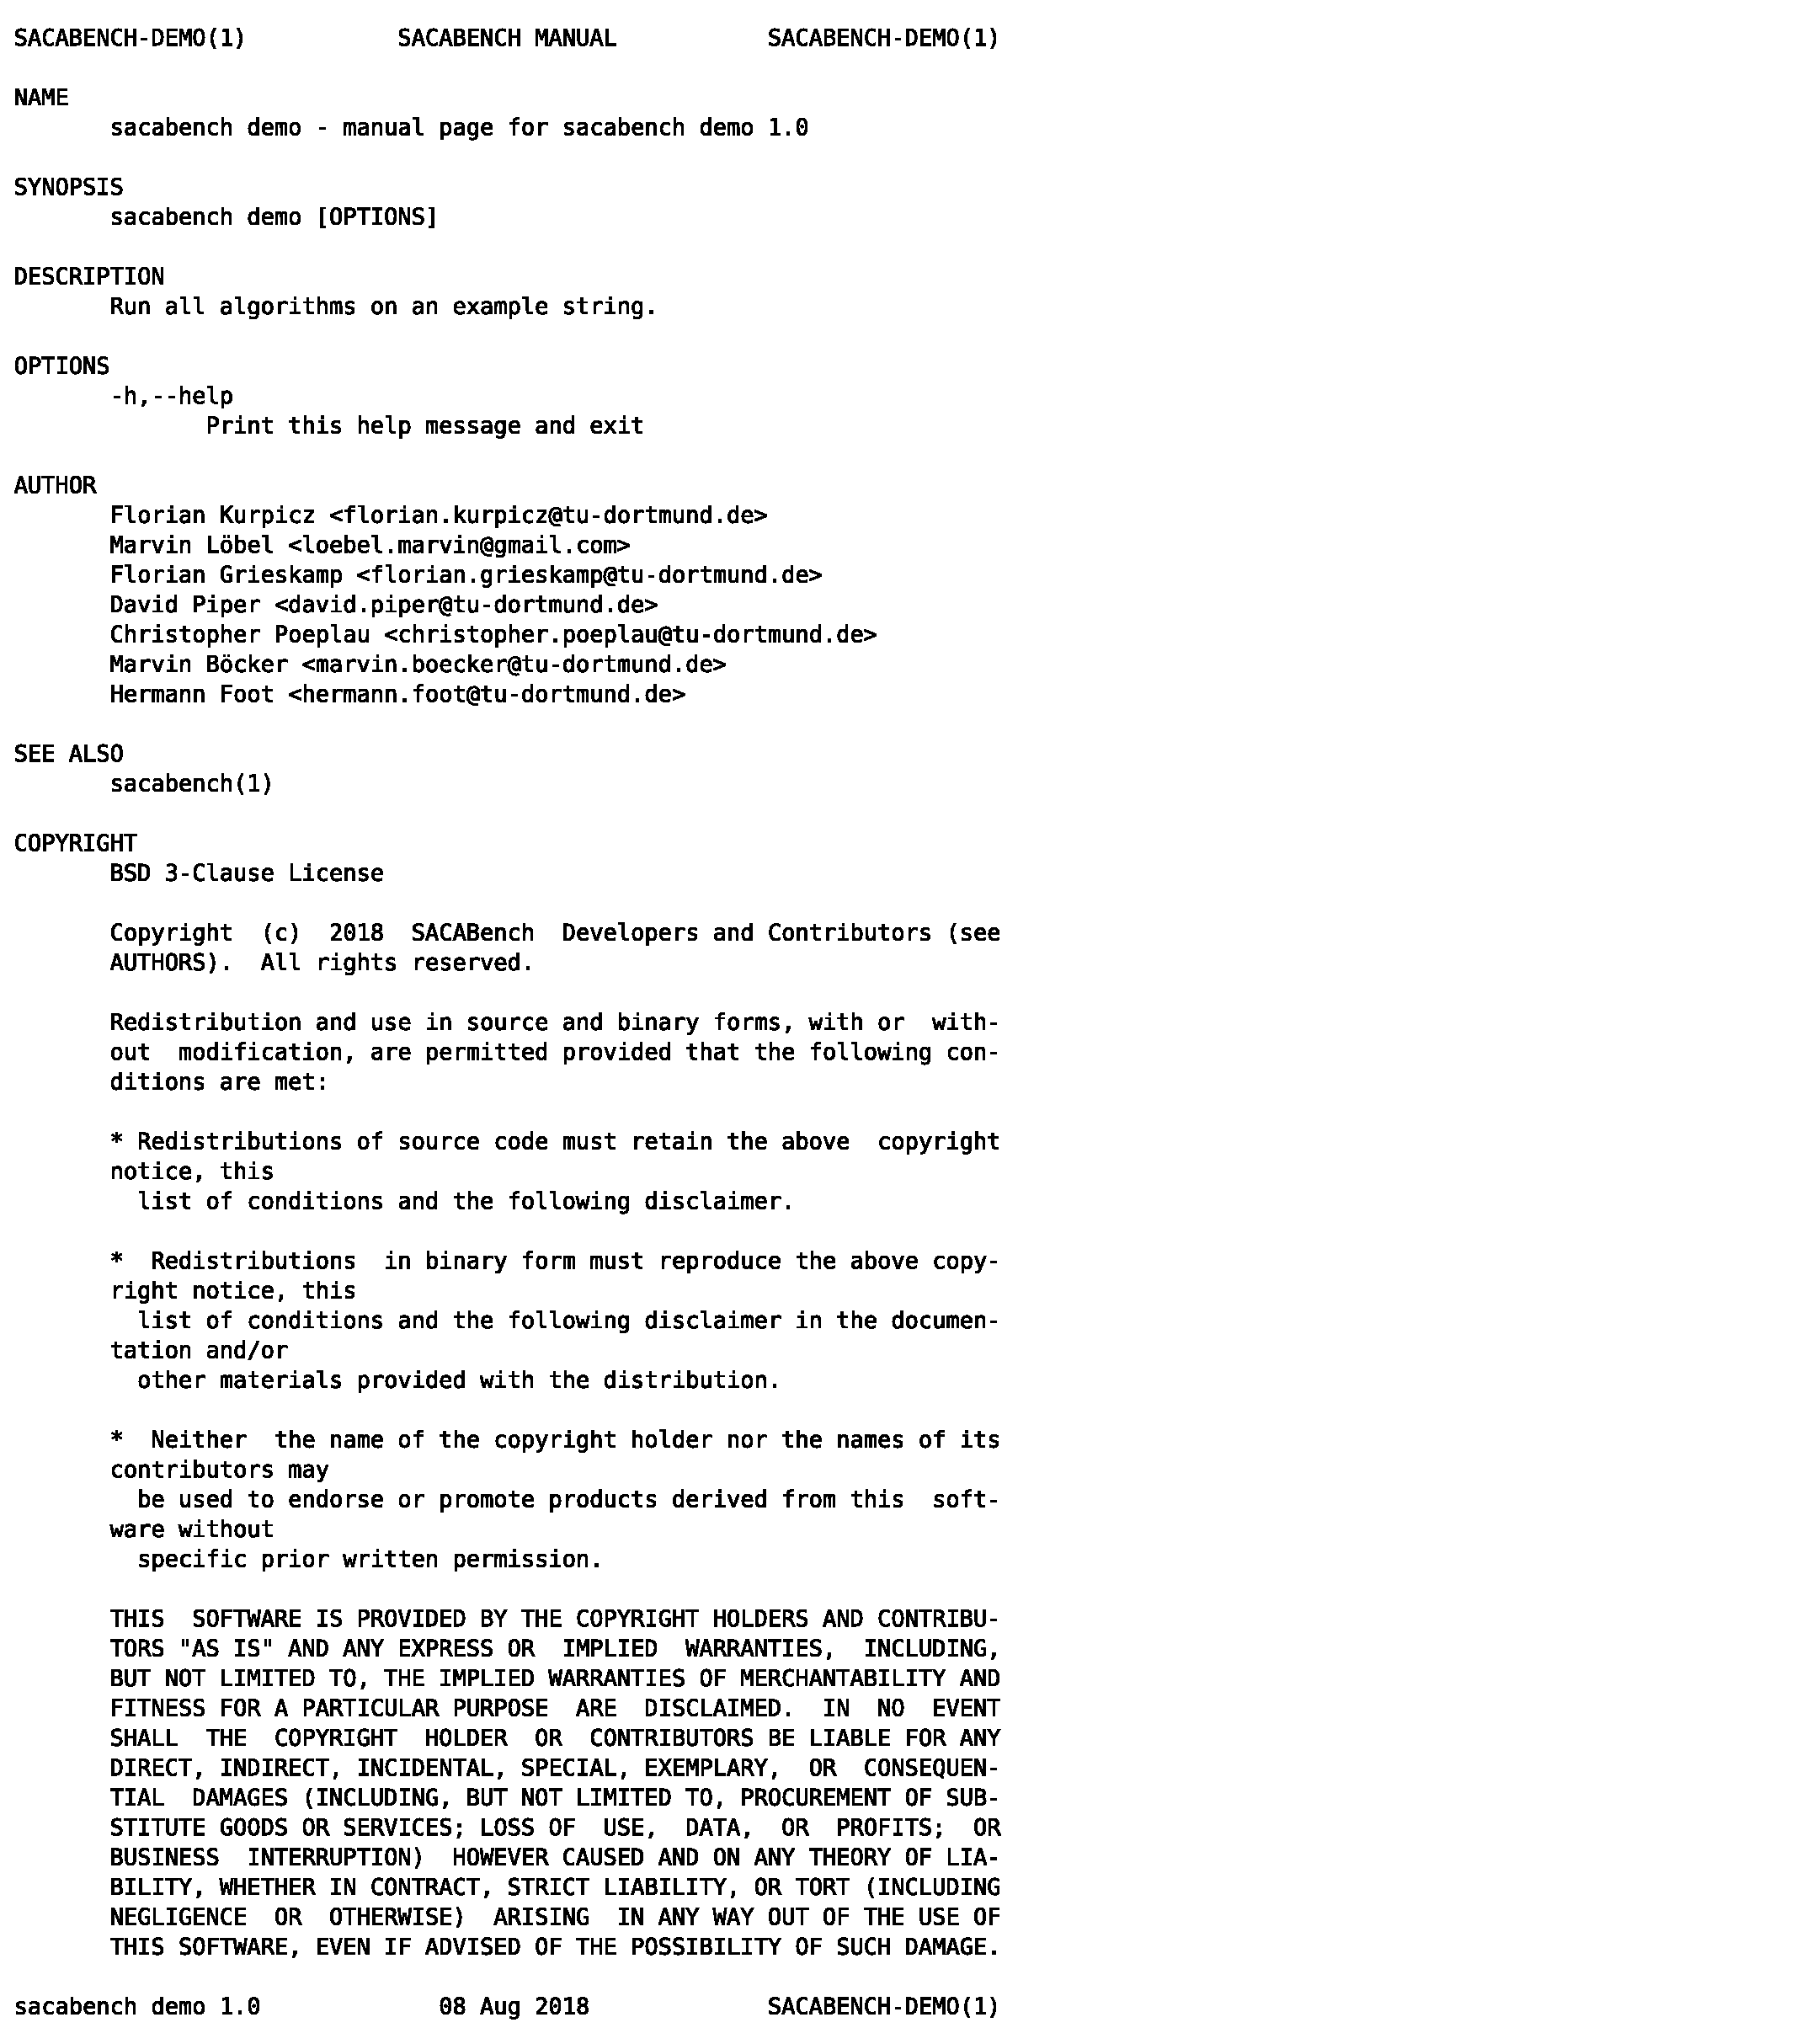
\includegraphics[page=1, viewport=0cm 32.8cm 20.5cm 41.0cm, clip, width=.5\textwidth]{{kapitel/framework/cli/sacabench-demo/sacabench-demo}.pdf}\\
    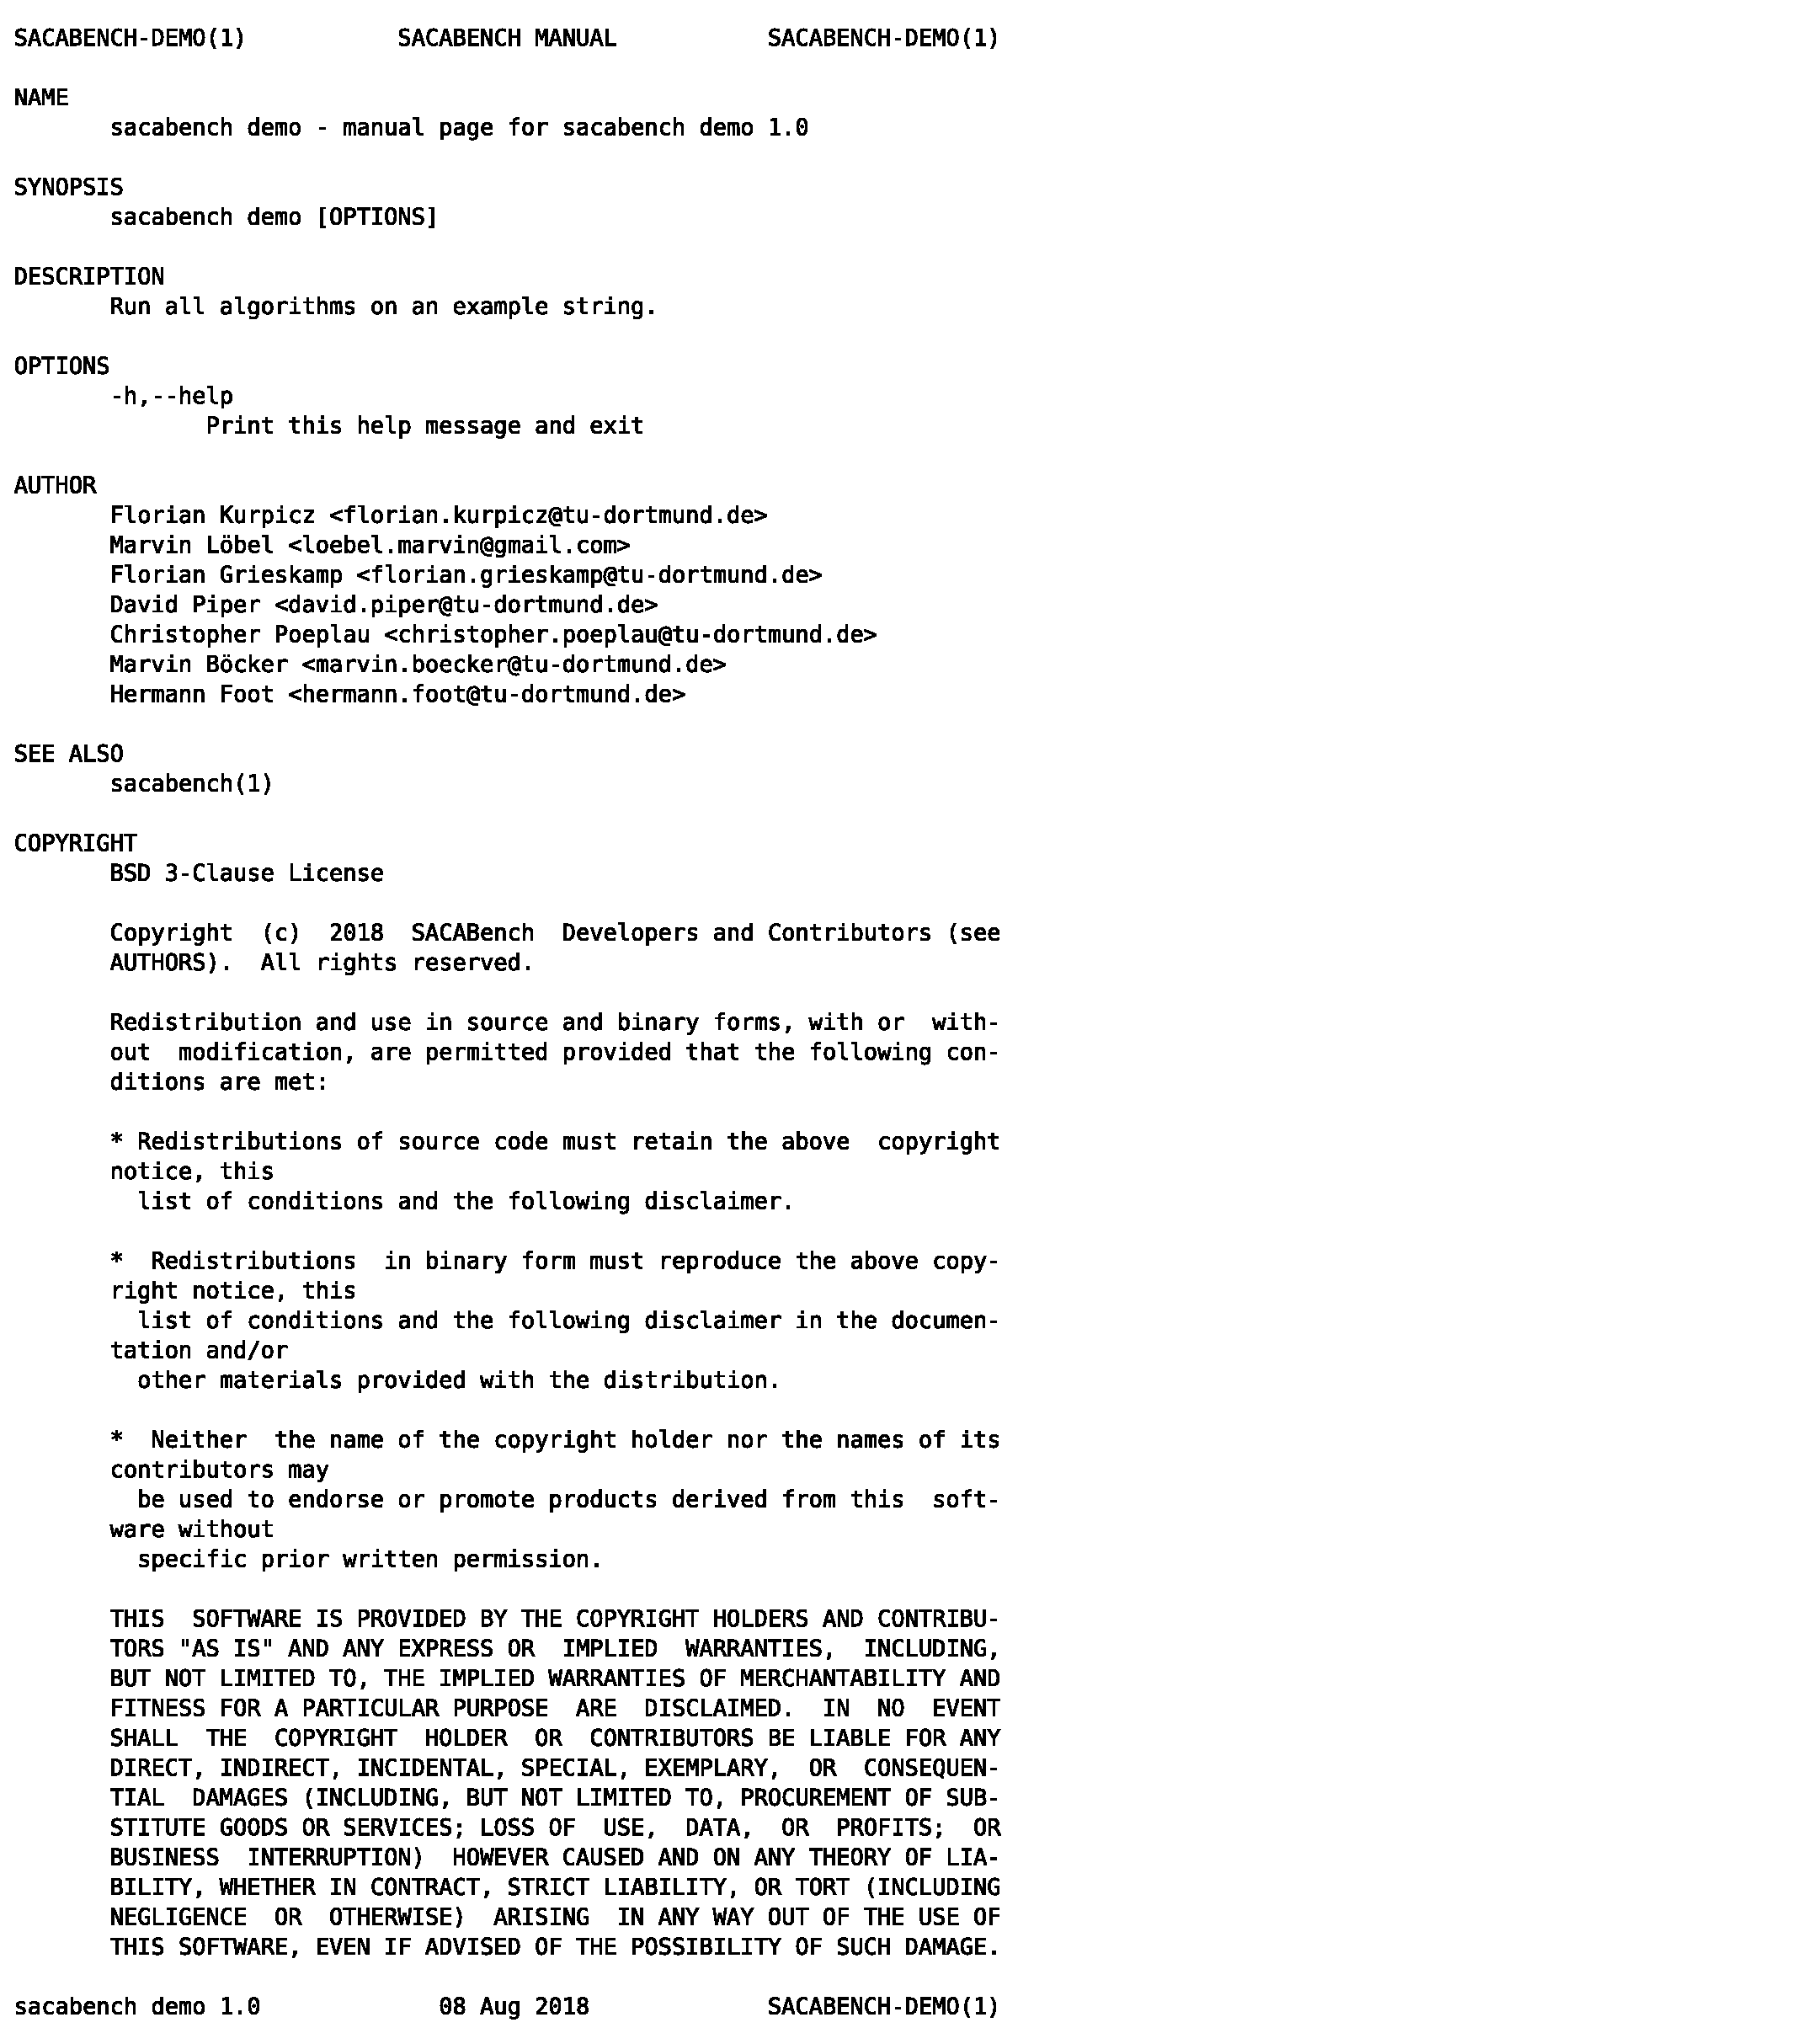
\includegraphics[page=1, viewport=0cm 25cm 20.5cm 26.3cm, clip, width=.5\textwidth]{{kapitel/framework/cli/sacabench-demo/sacabench-demo}.pdf}\\
    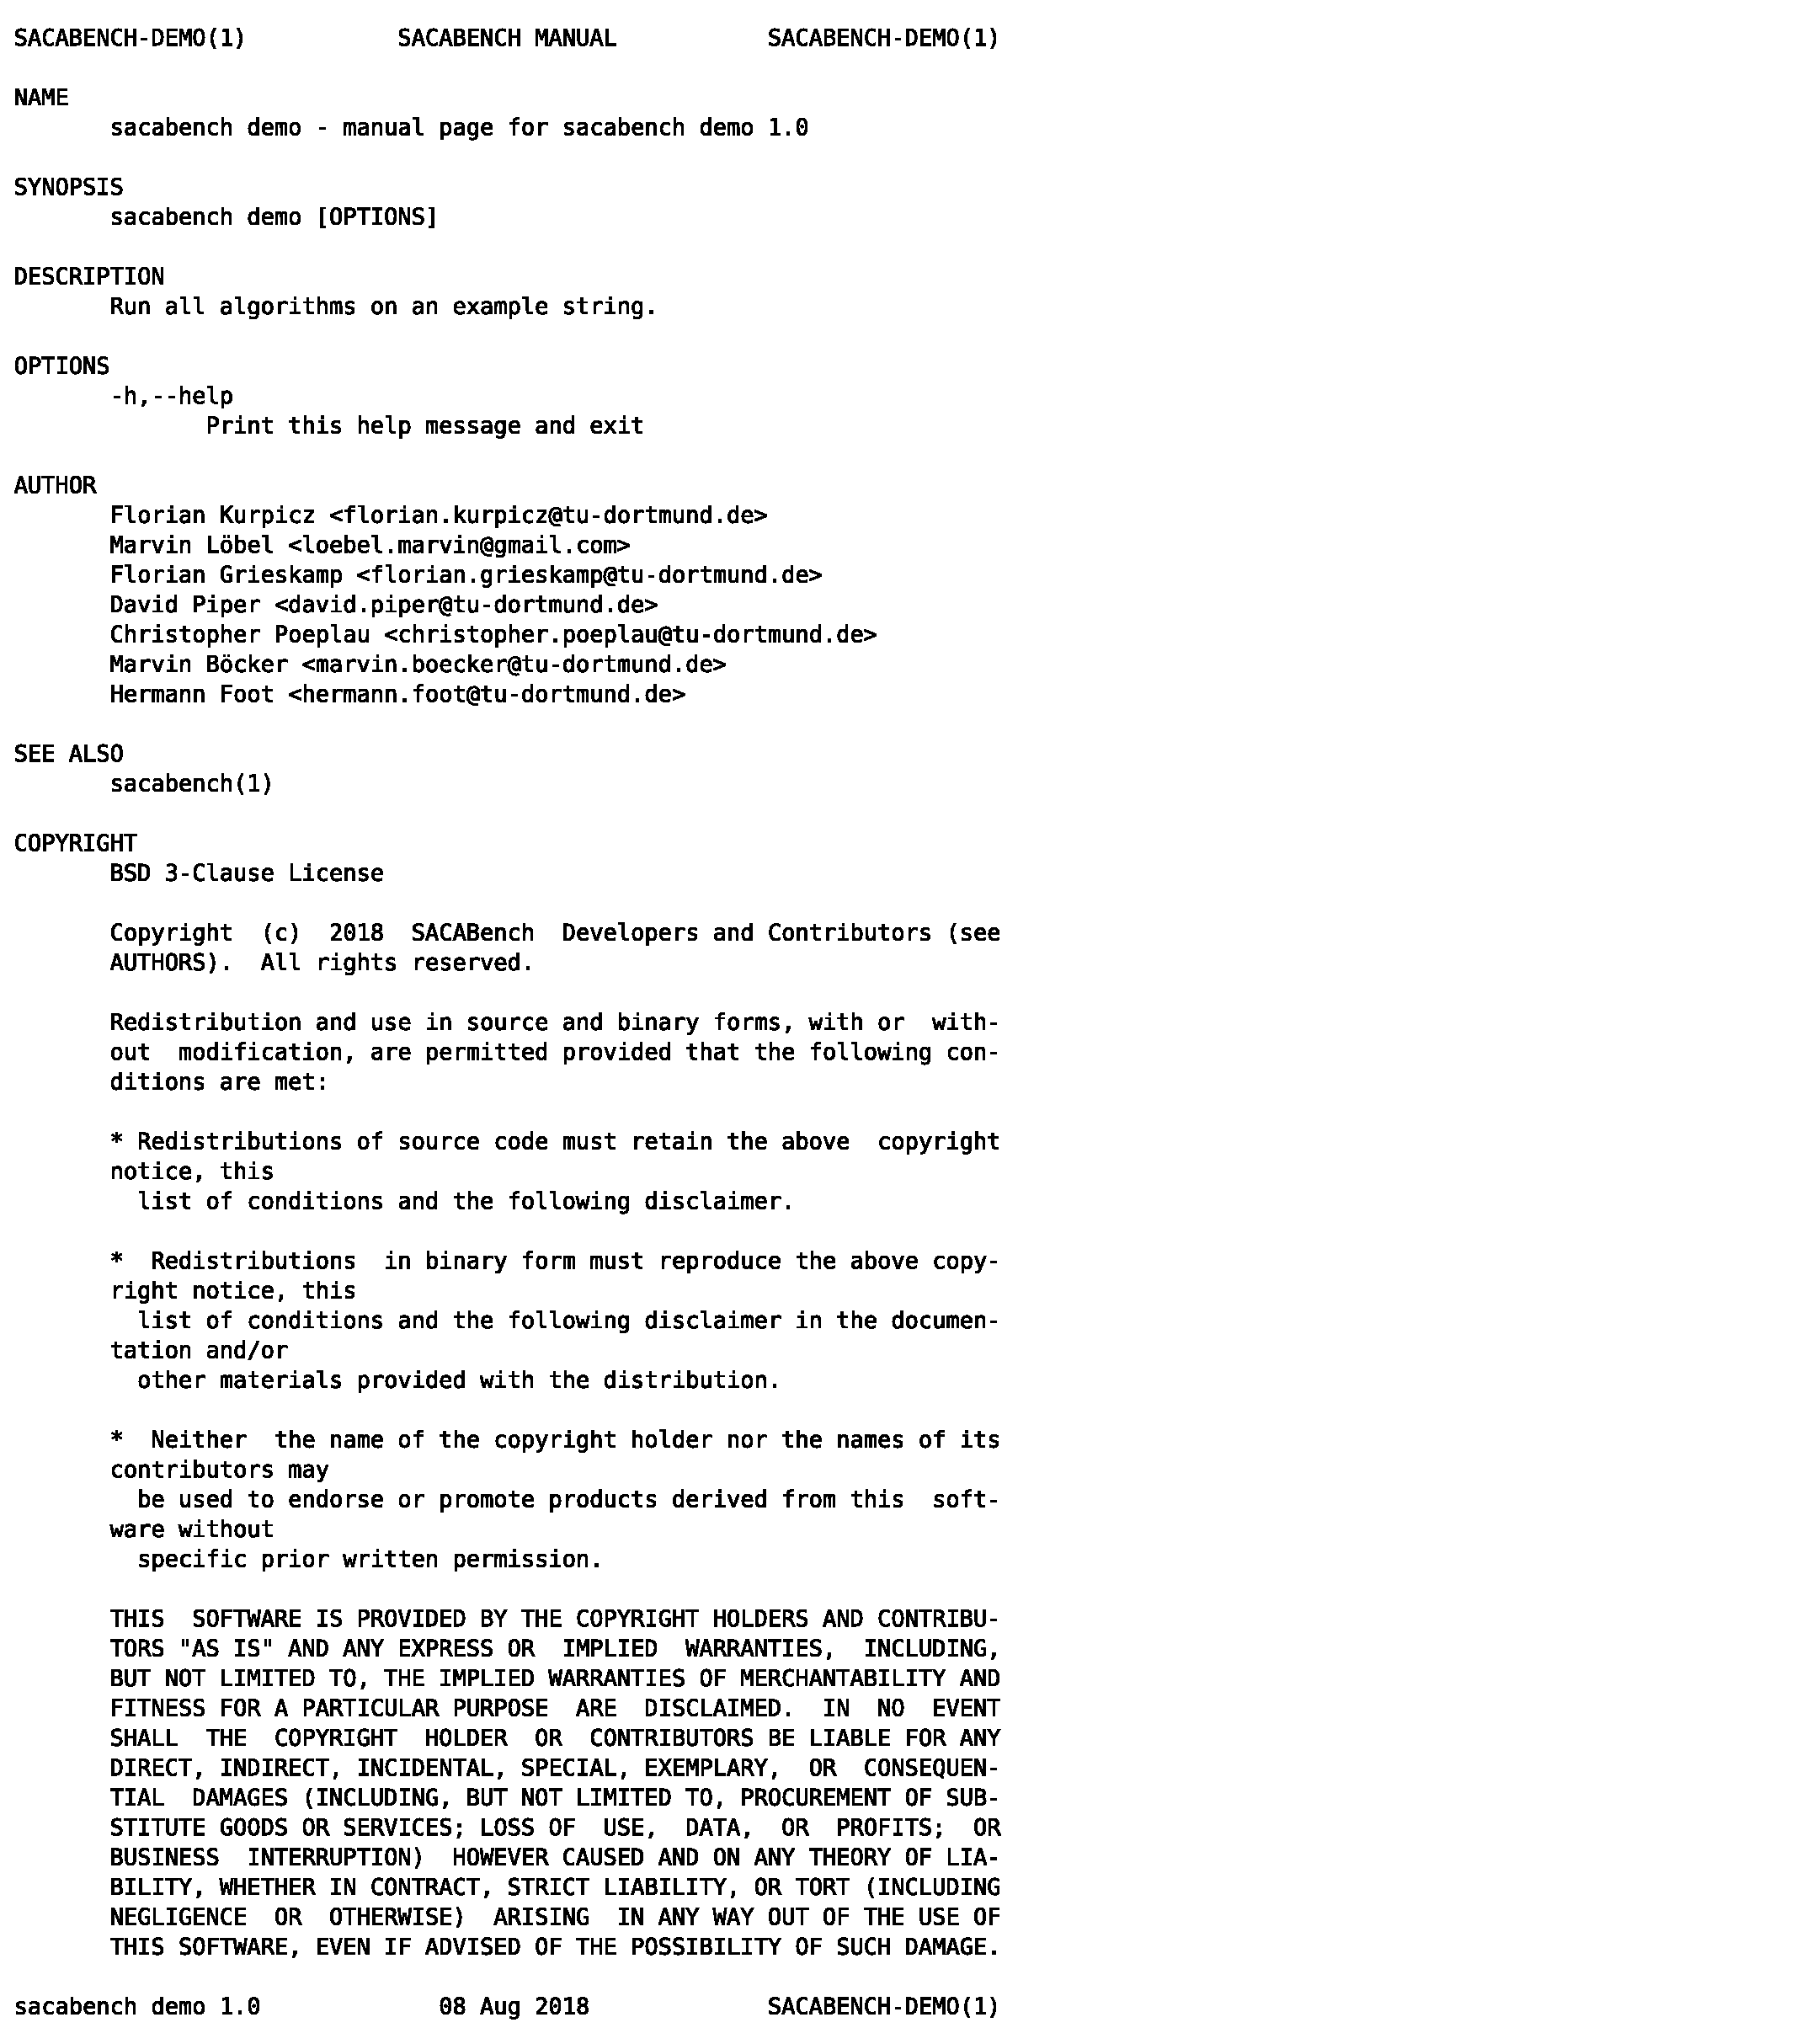
\includegraphics[page=1, viewport=0cm 0cm 20.5cm 1.5cm, clip, width=.5\textwidth]{{kapitel/framework/cli/sacabench-demo/sacabench-demo}.pdf}
    \caption{gekürzte Ausgabe von \texttt{man sacabench demo}}
    \label{manpage:sacabench-demo}
\end{wrapfigure}
Mit dem Befehl \texttt{sacabench demo} können alle Algorithmen auf einem kurzen Beispieltext (\glqq \termfont{hello world}\grqq) ausgeführt werden.\par
Diese Funktionalität erfüllt ausschließlich den Zweck, das Framework sowie die Algorithmen auf Lauffähigkeit auf dem verwendeten System zu testen. Auch hier ist eine Hilfeoption über \termfont{-h} bzw. \termfont{-{}-help} erreichbar.\par
}
